\section{Circuito construido}
\subsection{Componentes utilizados}
El circuito que se construyó es el de la figura 13, para su implementación física, se utilizaron los siguientes componentes:
\begin{itemize}
    \item Placa de fenólico simple faz 5x5.
    \item 2 BNC hembra
    \item Alambre de cobre esmaltado de 1 mm de diámetro
    \item \(C_1 = 33\) pF
    \item \(C_2 = 271\) pF
    \item \(C_3 = 47\) pF
    \item \(C_4 = 50\) pF (Se utilizaron dos capacitores en serie de 100 pF)
    \item \(R_L = 1\) k\(\Omega\)
\end{itemize}
\begin{figure}[!h]
    \centering
    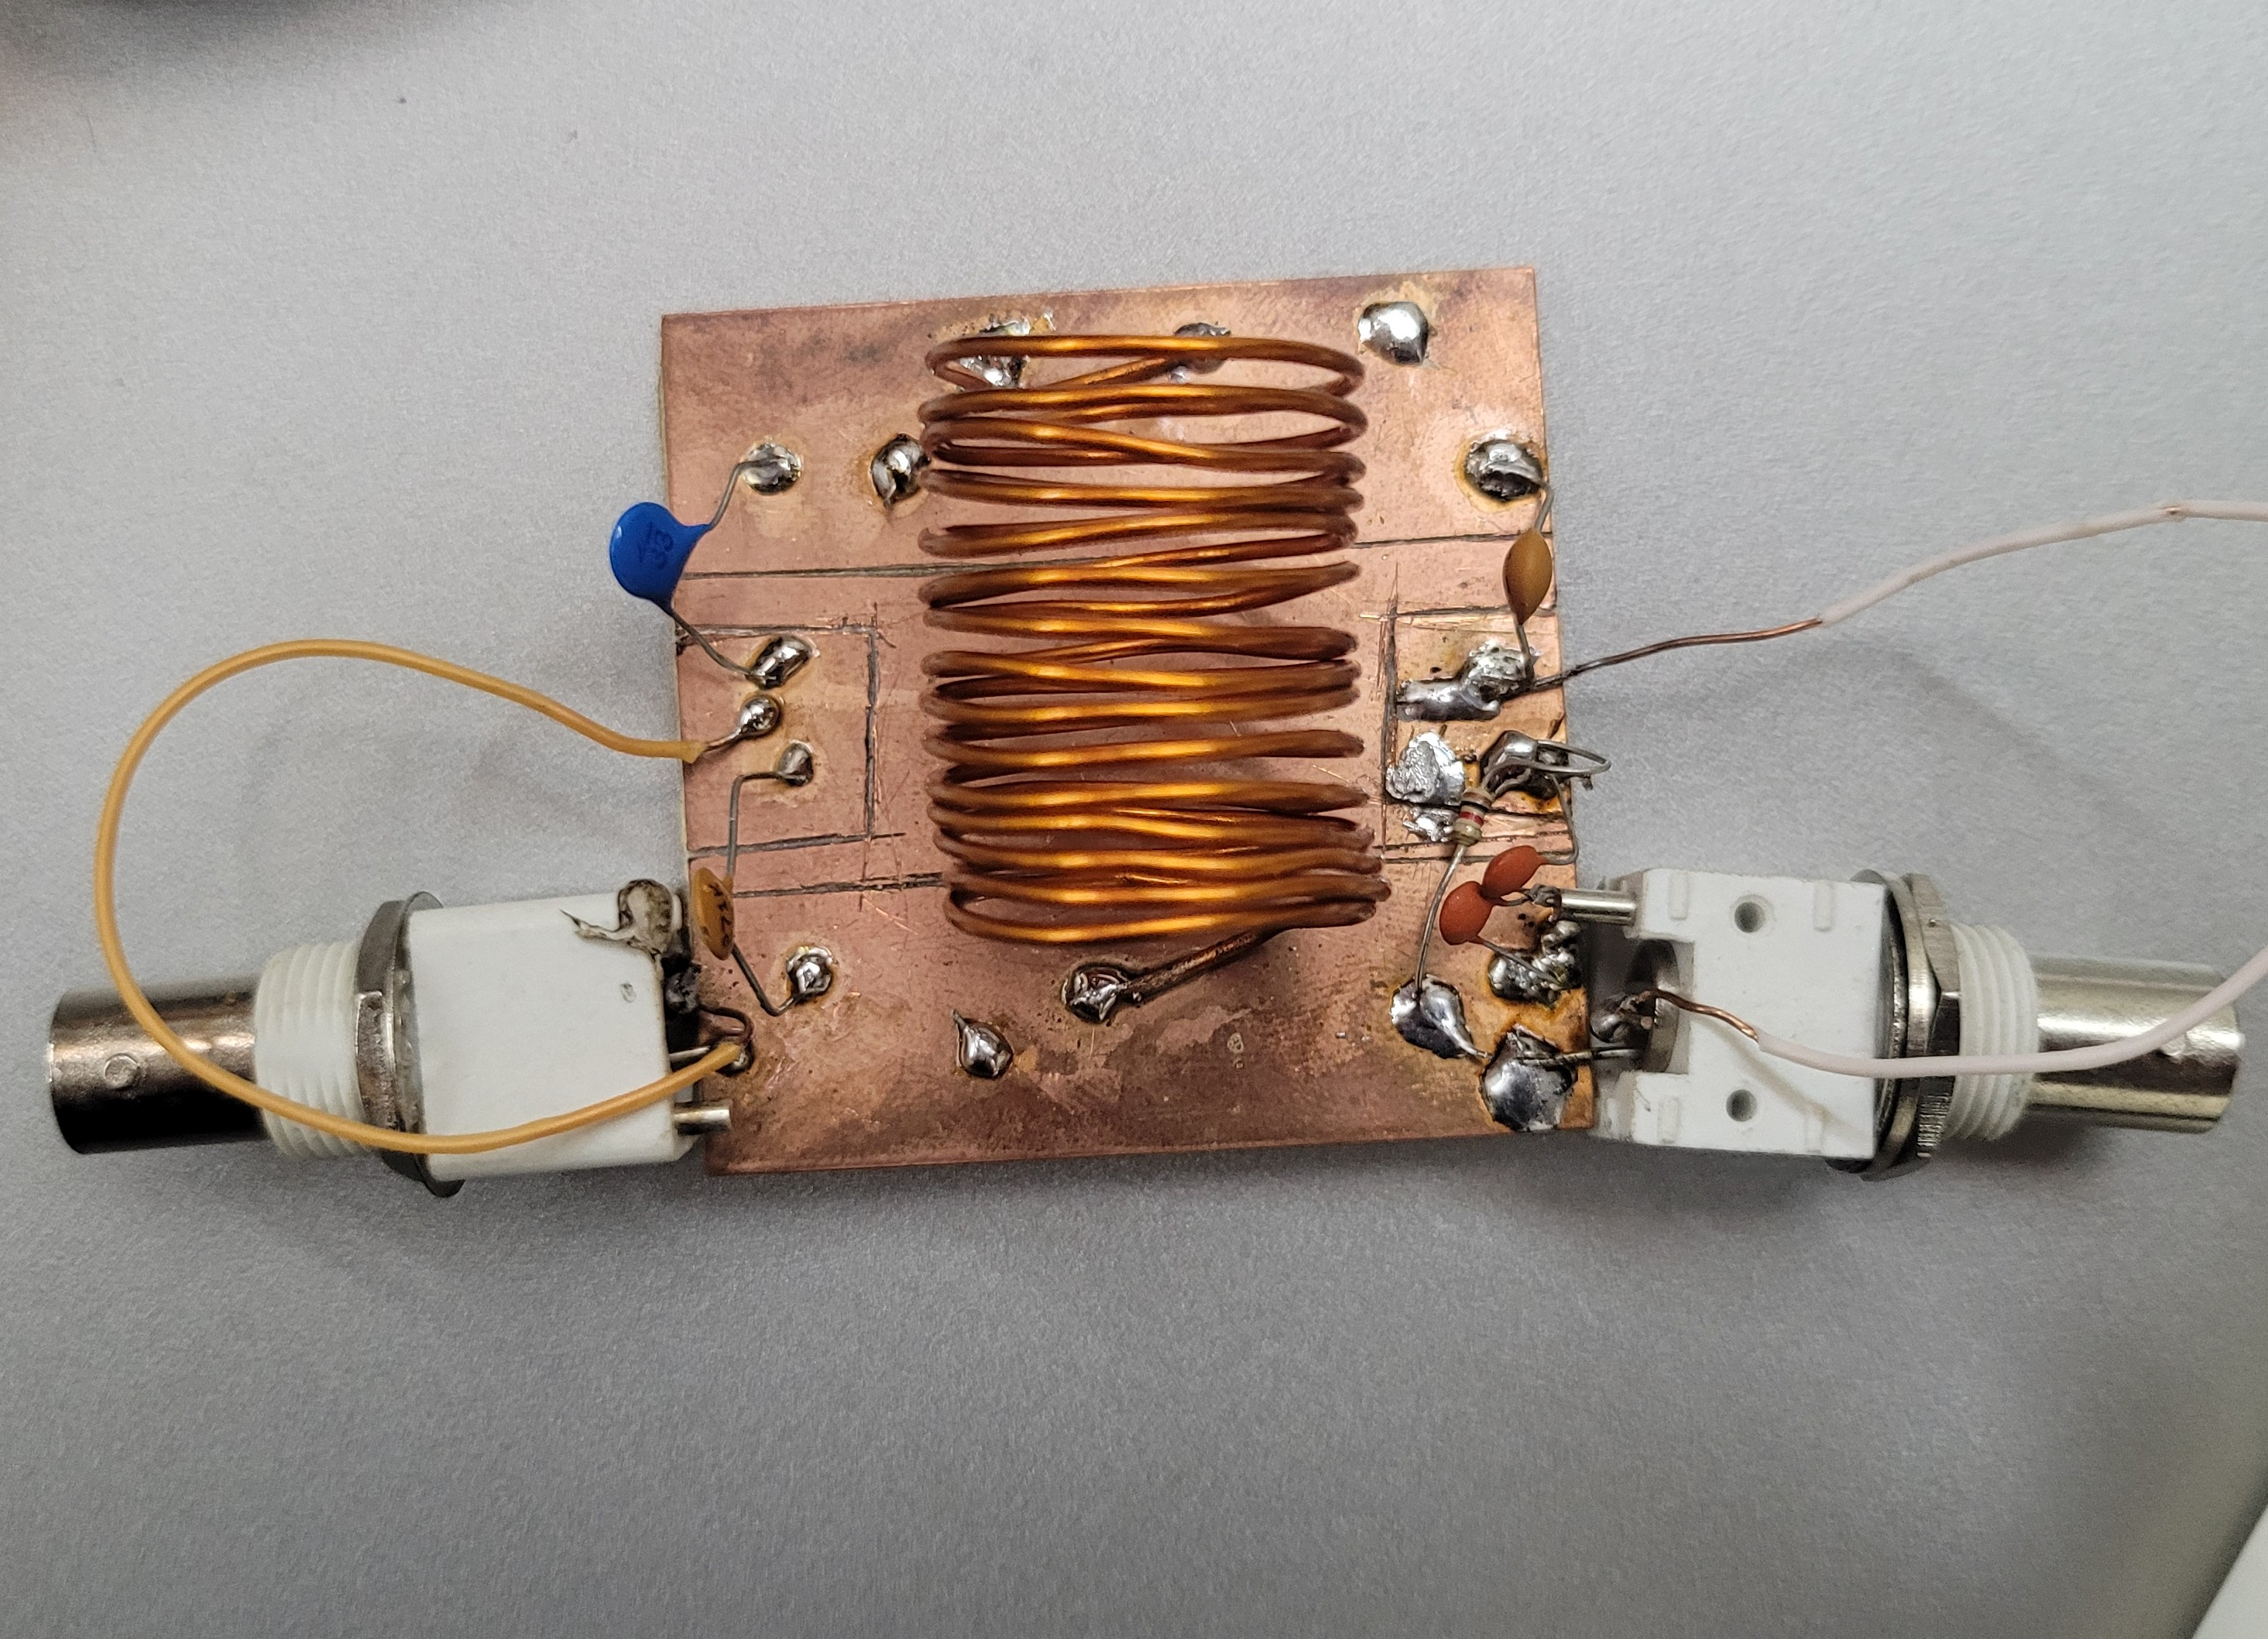
\includegraphics[scale=0.1]{Imagenes/Circuito montado.jpg}
    \caption{Circuito construido}
    \label{fig:Circteo__}
\end{figure}
Se calculó la capacidad total de la siguiente forma:
\begin{equation}
    C_T = (C_1//C_2)+(C_3//C_4) = 29,44pF + 24,22pF = 53,66 \,\ \text{pF}
\end{equation}

\newpage
\subsection{Mediciones}
\subsubsection{Circuito conectado a tope}
\begin{figure}[!h]
    \centering
    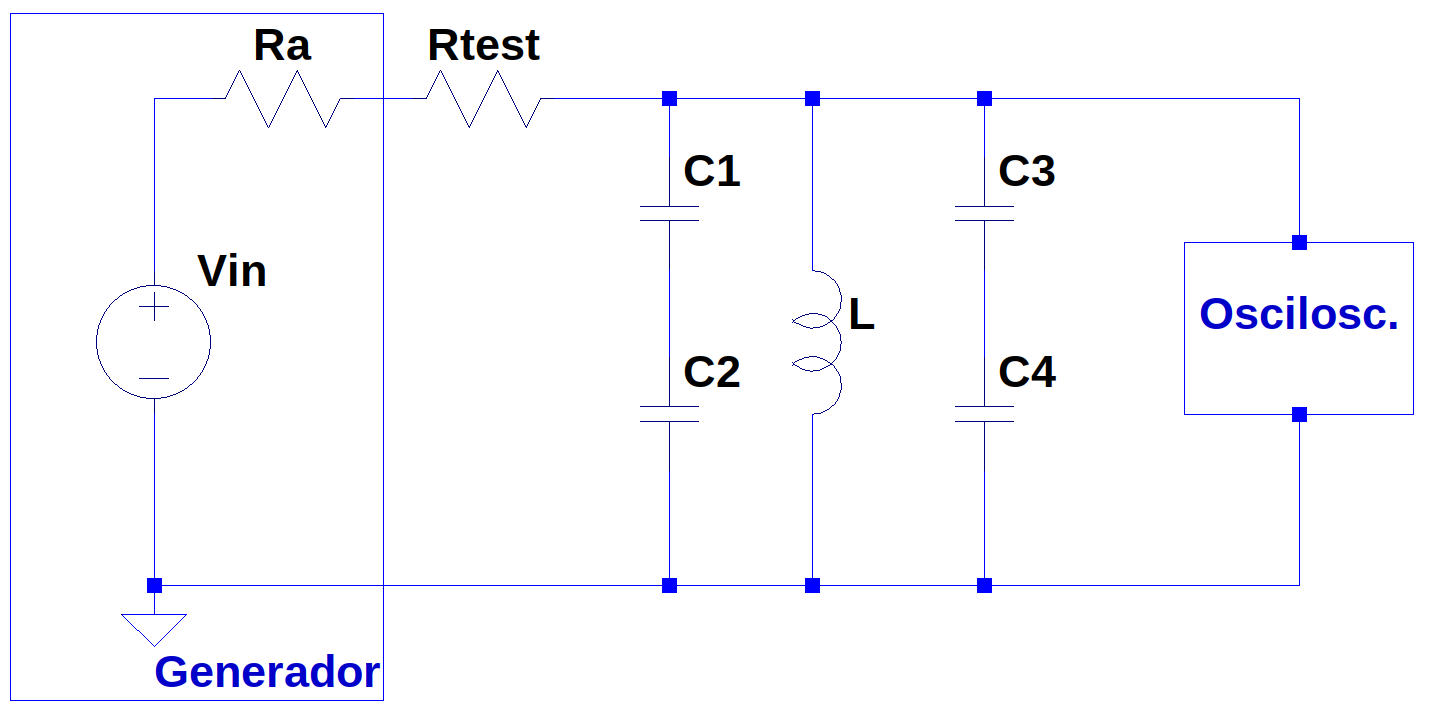
\includegraphics[scale=0.3]{Imagenes/Circuito conectado a tope.png}
    \caption{Circuito conectado a tope}
    \label{fig:Circtope}
\end{figure}
Para esta configuración se agrega \(R_t_e_s_t = 1\)k\(\Omega\) y los instrumentos se conectaron como se observa en la figura 16.
En este tipo de conexión, se realizaron 3 mediciones: \(f_o_1\), \(f_o_2\), \(R_p\).

La \(f_o\) no es posible medirla de manera directa debido a todas las capacidades parásitas que se agregan al circuito al realizar las mediciones, tanto los conectores, cables y el mismo osciloscopio agregan capacidades al circuito que afectan la capacidad total del circuito y esto modifica la frecuencia de resonancia del mismo. El método que se utilizó para calcular \(f_o\) es despejarlo a partir de  las dos mediciones \(f_o_1\) y \(f_o_2\)\ %mediante la medicion de dos frecuencias de resonancias, \(f_o_1\) tal como se observa en la figura 12 y \(f_o_2\) agregando un capacitor conocido \(C_F\) en paralelo a la bobina, el cual es de 18 pF.

Para medir la \(f_o_1\), se buscó el valor donde resonaba el circuito, es decir, donde su amplitud en tensión era máxima:
\begin{equation}
    f_o_1 = 7,8 \,\ \text{MHz} 
\end{equation}

En esta misma medición, se observo que amplitudes se tenían, la del generador y la señal que mide el osciloscopio a la salida del circuito:

\begin{align}
    V_{\mathrm{gen}} &= 3.64 \, \mathrm{V_{pp}} \\
    V_{\mathrm{out}} &= 3.40 \, \mathrm{V_{pp}}
\end{align}

Luego, para la medición de \(f_o_2\) se agregó un capacitor \(C_F = 18\) pF en paralelo a la bobina para con esto modificar la frecuencia de resonancia:

\newpage
\begin{figure}[!h]
    \centering
    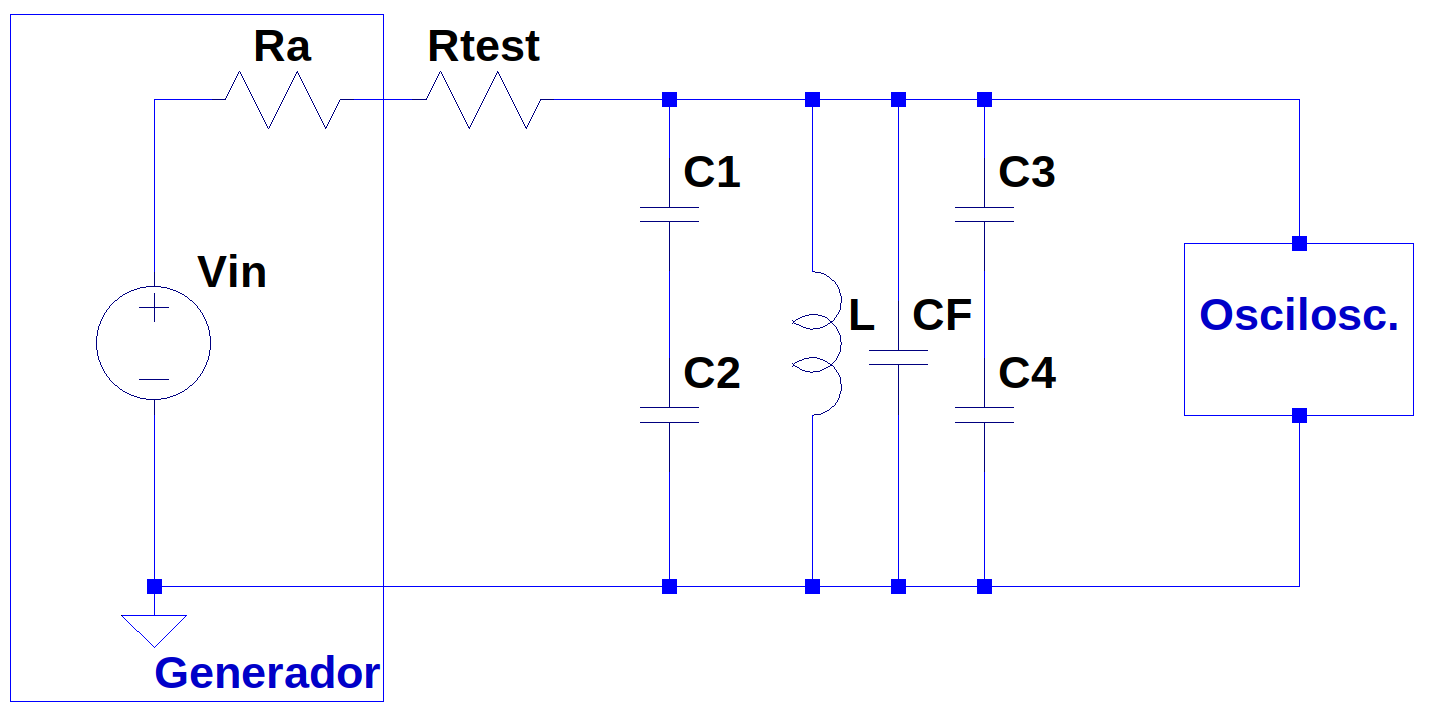
\includegraphics[scale=0.3]{Imagenes/CF.png}
    \caption{Capacitor \(C_F\) en paralelo a la bobina}
    \label{fig:Circtope}
\end{figure}
Se buscó nuevamente la frecuencia de resonancia con esta modificación y se obtuvo:
\begin{equation}
    f_o_2 = 7,43 \,\ \text{MHz} 
\end{equation}

Por lo tanto, lo siguiente fue encontrar las capacidades parásitas \(C_X\), el cual se encuentra en paralelo en ambos circuitos. Para ello, se utiliza la ecuación (1):

\begin{equation}
    f_o_1 = \frac{1}{2\pi \sqrt{(C_T+C_X)L}} = 7,8 \,\ \text{MHz}
\end{equation}

\begin{equation}
    f_o_2 = \frac{1}{2\pi \sqrt{(C_T+C_X+C_F)L}} = 7,43 \,\ \text{MHz}
\end{equation}
\begin{gather}
    \left(\frac{f_{o1}}{f_{o2}}\right)^2 = \frac{(2 \pi)^2 (C_T+C_X+C_F)L}{(2 \pi)^2 (C_T+C_X)L} \notag \\
    \left(\frac{f_{o1}}{f_{o2}}\right)^2 = \frac{C_T+C_X+C_F}{C_T+C_X} \notag \\
    \hspace{2.5em} C_X\left[\left(\frac{f_{o1}}{f_{o2}}\right)^2-1\right]+C_T\left(\frac{f_{o1}}{f_{o2}}\right)^2 =C_T+C_F \notag \\
    C_X =\frac{C_T((f_o_2)^2-(f_o_1)^2)+C_F (f_o_2)^2}{(f_o_1)^2-(f_o_2)^2} \label{eq:conjunto}
\end{gather}
Reemplazando se obtuvo:
\begin{equation}
    C_X = 122,68 \,\ \text{pF}
\end{equation}

Se utilizó la ecuación (32) para despejar L:

\begin{equation}
    L = \frac{1}{(2\pi\cdot7,8\text{MHz})^2}\cdot\frac{1}{53,66pF+122,68pF} = 2,36 \,\ \mu\text{Hy}
\end{equation}

\newpage

Con \(L\), se tienen todos los valores necesarios para calcular la frecuencia de resonancia.

\begin{equation}
    f_o = \frac{1}{2\pi \cdot \sqrt{LC}} = \frac{1}{2\pi \cdot \sqrt{2,36\mu \text{Hy}\cdot 53,6\text{pF}}} = 14,14 \,\ \text{MHz}
\end{equation}

Finalmente, queda calcular \(R_p\), este se calcula a partir de los valores de tensión obtenidos en la medición de \(f_o_1\), el circuito equivalente de análisis es el siguiente:

\begin{figure}[!h]
    \centering
    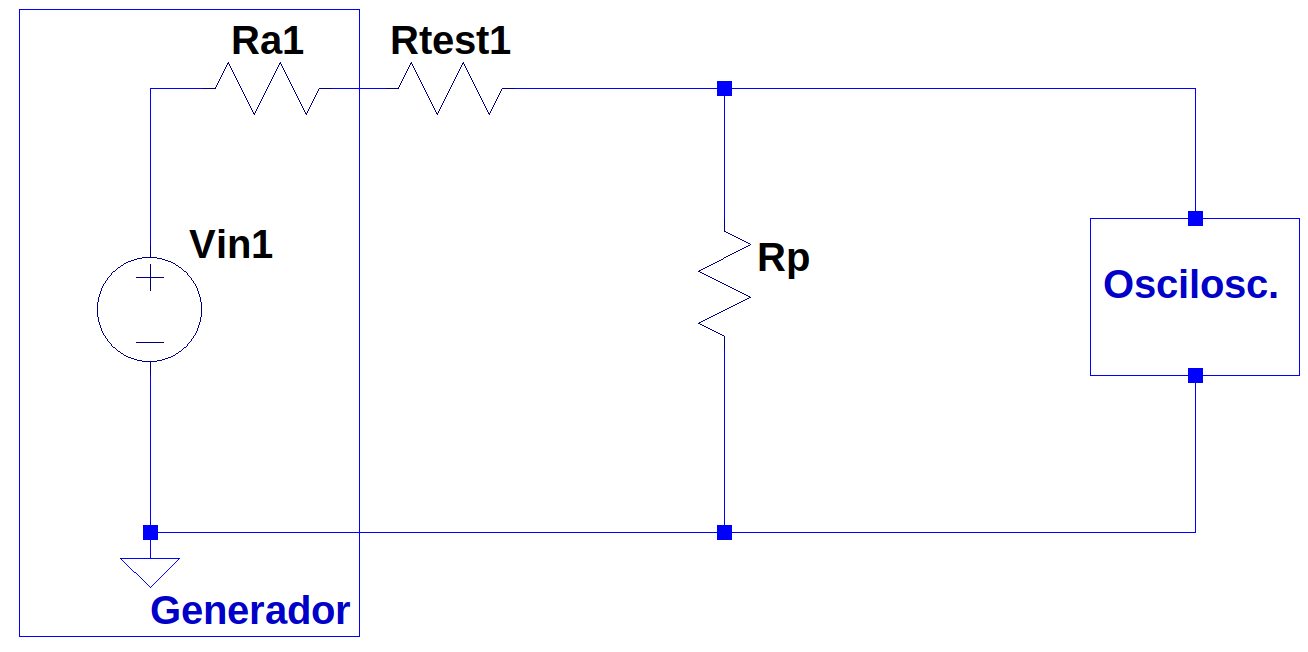
\includegraphics[scale=0.3]{Imagenes/RP.png}
    \caption{Circuito equivalente para medir \(R_p\)}
    \label{fig:Circrp}
\end{figure}

Se plantea un divisor de tensión, del cual se despeja \(R_p\):
\begin{equation}
    V_o_u_t = V_g_e_n\frac{R_p}{R_p+R_a+R_t_e_s_t} 
\end{equation}
De la ecuación (29) y (30) se utilizaran los valores de tensión.
\begin{equation}
    3,40V = 3,64V\frac{R_p}{R_p+50\Omega+1k\Omega} 
\end{equation}

\begin{equation}
    R_p = \frac{R_a+R_t_e_s_t}{(\frac{V_g_e_n}{V_o_u_t})-1} = \frac{50\Omega+1k\Omega}{(\frac{3,64V}{3,40V})-1} = \boxed{14,88 \,\ k\Omega}
\end{equation}

Con \(R_p\) se calcula \(Q_d\):

\begin{equation}
    Q_d = \frac{R_p}{X_L} = \frac{14,88k\Omega}{2\pi \cdot 14 \text{MHz} \cdot 2,3\mu \text{Hy}} = \boxed{73,54} 
\end{equation}

\newpage

\subsubsection{Circuito conectado al punto medio}

\begin{figure}[!h]
    \centering
    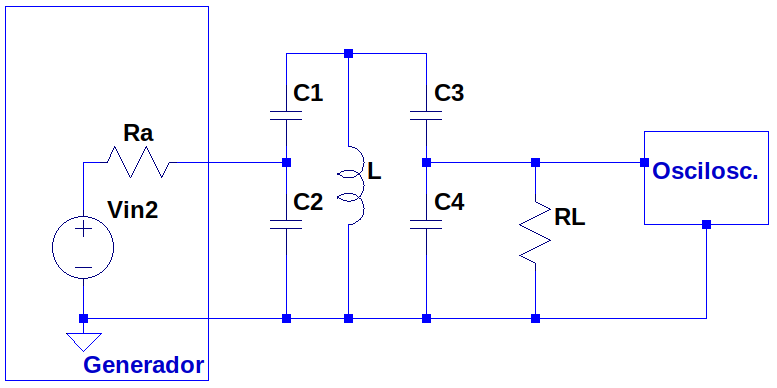
\includegraphics[scale=0.4]{Imagenes/Circptomedio.png}
    \caption{Circuito conectado al punto medio}
    \label{fig:Circrp}
\end{figure}

Para esta configuración se desconecto \(R_t_e_s_t\) y se conectó \(R_L\). Como también las conexiones del generador y osciloscopio se conectaron de la forma que se observa en la figura 19.

En esta configuración se realizaron todas las mediciones faltantes: \(BW\), \(Z_i_n\), \(Z_o_u_t\), \(Q_c\).

Para la medición de \(BW\) se buscó la resonancia del circuito, la cual, como es de esperar, es una frecuencia de resonancia distinta a las anteriores. Por lo tanto, se realizó un barrido en frecuencia hasta encontrar el valor de tensión máximo:


\begin{equation}
    V_o_u_t = 3,88 \,\ V_p_p
\end{equation}

\begin{equation}
    f_o_4 = 12,13 \,\ \text{MHz}
\end{equation}



Luego, se buscaron los valores de tensión para los cuales caen 3 dB lo que es equivalente a la siguiente ecuación:
\begin{equation}
    V_f_c = 3,88 \,\ V_p_p \cdot 0,707 = 2,74 \,\ V_p_p
\end{equation}

Por lo tanto, se buscó la frecuencia de corte superior e inferior para dicho valor de tensión.

\begin{equation}
    f_c_l = 11,95 \,\ \text{MHz}
\end{equation}

\begin{equation}
    f_c_h = 12,39 \,\ \text{MHz}
\end{equation}

Con los valores encontrados de frecuencia, se calculó el BW:

\begin{equation}
BW = 12,39 - 11,95 = \boxed{0,44 \,\ \text{MHz}}
\end{equation}

Con \(BW\) se calculó \(Q_c\) con la ecuación (3):
\begin{equation}
    Q_c= \frac{14,14 \,\ \text{MHz}}{0,44 \,\ \text{MHz}} = \boxed{32,13}
\end{equation}

\newpage
La siguiente medición es \(Z_i_n\), para lo cual, se van a medir valores de tensión a la entrada, la disposición es la siguiente:

\begin{figure}[!h]
    \centering
    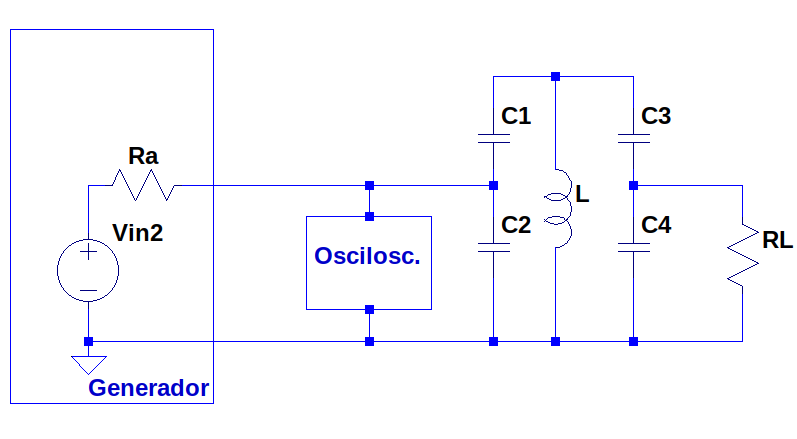
\includegraphics[scale=0.4]{Imagenes/ZIN.png}
    \caption{Medición de \(Z_i_n\)}
    \label{fig:Zin}
\end{figure}

De esta forma, la medición consiste en observar como cae la tensión del generador al conectar el circuito como se observa en la figura 20, si este cae a la mitad, el circuito se encontraría adaptado:

\begin{equation}
    V_g_e_n = 3,28 \,\ V_p_p
\end{equation}

Luego, se mide la caída de tensión:

\begin{equation}
    V_o_s_c = 1,32 \,\ V_p_p
\end{equation}

\begin{equation}
   V_o_s_c  = V_g_e_n \cdot \frac{Z_i_n}{Z_i_n+R_a} 
\end{equation}

Despejando \(Z_i_n\) de la ecuación (51):
\begin{equation}
    Z_i_n = R_a \frac{V_o_s_c}{V_g_e_n-V_o_s_c} = 50\Omega \frac{1,32V}{3,28V-1,32V} = \boxed{33,67 \Omega}
\end{equation}

\newpage
La siguiente medición es \(Z_o_u_t\), para la cual se deben realizar dos mediciones. Una medición se realizó como esta dispuesto en la figura 19, que es la medición con el circuito cargado y luego otra medición es desconectando la carga \(R_L\), es decir, descargado.

\begin{figure}[!h]
    \centering
    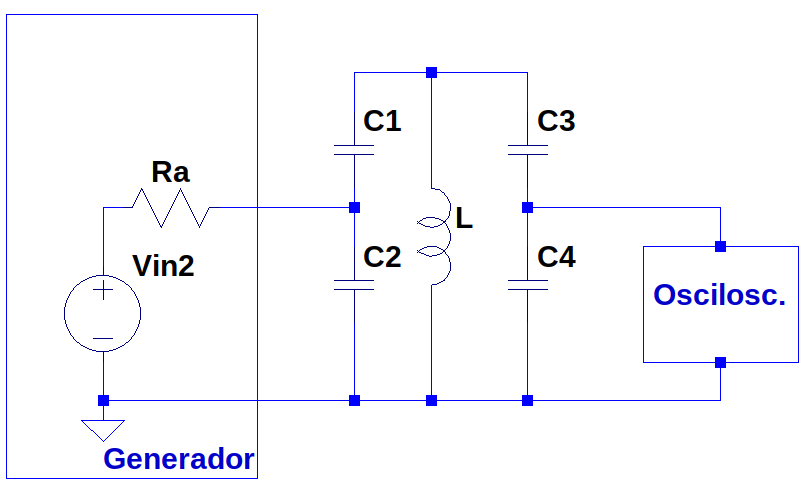
\includegraphics[scale=0.4]{Imagenes/Zout.png}
    \caption{Medición de \(Z_o_u_t\) descargado}
    \label{fig:Zin}
\end{figure}

Los valores que se obtuvieron del osciloscopio son las tensiones, por un lado la tensión de salida con el circuito cargado \(V_L\) y con el circuito descargado \(V_o_u_t\).

\begin{equation}
    V_L = 5,84 V
\end{equation}

\begin{equation}
    V_o_u_t = 6,96 V
\end{equation}

Luego, se plantea un divisor de tensión similar al que se planteó en la ecuación (51)

Por lo que se calcula \(Z_o_u_t\) de la siguiente manera:

\begin{equation}
    Z_o_u_t = R_L \frac{V_o_u_t-V_i_n}{V_L} = 1k\Omega\frac{6,96V-5,84V}{5,84V} = \boxed{191,78\Omega}
\end{equation}


